\documentclass[t]{beamer}

%\documentclass[handout, t]{beamer}
\setbeamertemplate{navigation symbols}{}
\usepackage{pstricks}
\usepackage{mathtools}
\usepackage{amsfonts}
\usepackage{mathrsfs}
\usepackage{amsmath}
\setbeamertemplate{navigation symbols}{}
\usepackage{bm}
\usepackage[UTF8]{ctex}
\usetheme{AnnArbor}
\usefonttheme{serif}
\useinnertheme{rounded}
%\usecolortheme{crane}
\setbeamertemplate{blocks}[rounded][shadow=true]

\newcommand{\dif}{{\;\rm d}}
\usepackage{graphicx}
\usepackage{pgf}
\usepackage{tikz}
\usetikzlibrary{arrows, decorations.pathmorphing, backgrounds, positioning, fit, petri, automata}
\tikzset{>=stealth}


\setmainfont{Times New Roman}
\setCJKmainfont{Microsoft YaHei}


\hypersetup{pdfpagemode=FullScreen}
\renewcommand{\Pr}{\mathbb{P}}
\usepackage{blkarray}


\setbeamercolor{block title}{bg=red!10!white}
\setbeamercolor{block body}{bg=gray!10!white}

\usepackage{multicol}
\newcommand{\E}{\mathbb{E}}
\newcommand{\EP}{\mathbb{E}^{\mathbb{P}}}
\newcommand{\EQ}{\mathbb{E}^{\mathbb{Q}}}
\newcommand{\Var}{{\rm Var}}
\newcommand{\Cov}{{\rm Cov}}


\begin{document}
\fontsize{11}{18}\selectfont


\CTEXindent



  \title{第一章~~预备知识}
\author{随机过程及其在金融中的应用}
\date{中国人民大学出版社}
  \begin{frame}
    \maketitle
  \end{frame}

\begin{frame}{本章内容}
  \begin{multicols}{2}
    \tableofcontents
  \end{multicols}
\end{frame}

\section{事件与概率}
\subsection{样本和样本空间}
\begin{frame}{样本和样本空间}
  通常把按照一定想法去做的事件称为试验(experiment),把试验的可能结果称为样本点(sample
point),样本点的集合称为样本空间(sample space)
。
通常将样本空间记为$\Omega$,样本点记为$\omega$。

\begin{block}{举例:}
  一个均匀的骰子(dice)有六个面,每次抛出这个骰子,会得到相应的点数(比如:3)。这里“抛骰子”就是一个事件,也就是“试验”;
  在抛出骰子后得到的“点数”3就是“样本点”$\omega=3$;而骰子的可能点数为$1,2,3,\ldots,6$,因此对应的样本空间就是$\Omega=\{1,2,3,\ldots,6\}$。
\end{block}
  
  \end{frame}

  \subsection{事件与概率}
  \begin{frame}{事件与概率}
    事件(event)是样本空间$\Omega$的子集,且满足三个条件:
    \begin{enumerate}
      \item $\Omega$是事件;
      \item 若$A$是事件,则$A^c$是事件;
      \item 若$A_i$是事件,则$\bigcup\limits^{\infty}_{i=1}A_i$是事件。
    \end{enumerate}
  
\begin{block}{骰子的例子}
  如果“抛出的点数为3”是事件$A$,则其对立事件$A^c$就是“抛出的点数不为3”;另外,“抛一次骰子”是事件,则“抛无数次骰子”组成的所有事件的并集也是事件。
\end{block}

  \end{frame}


  \begin{frame}{事件}
    对于事件$A$,如果使用$\Pr(A)$表示事件发生的概率,则$\Pr(A)$满足以下条件:
    \begin{enumerate}
      \item 非负性:$\Pr(A)\ge 0$;
      \item 完备性:$\Pr(\Omega)=1$;
      \item 可列可加性:对于互不相容的事件$A_1,A_2,\ldots$,有:
      \begin{equation*}
    \Pr\left(\bigcup^{\infty}_{i=1}A_i\right)=\sum^{\infty}_{i=1}\Pr(A_i)
      \end{equation*}
    \end{enumerate}
  
  \end{frame}
  \subsection{概率空间}
  \begin{frame}{概率空间}
    对于样本空间$\Omega$和概率$\Pr$,用$\mathcal{F}$表示全体事件时,称三位一体的$(\Omega,\mathcal{F},\Pr)$为概率空间(probability
    space)。
    $\mathcal{F}$称作$\sigma$-代数(sigma-algebra),相当于样本空间$\Omega$的子集的集合。
  
    \begin{block}{举例:}
      假设样本空间$\Omega=\{1,2,3\}$,则
$\mathcal{F}$可表示为:
\begin{equation*}\mathcal{F}=\Big\{\emptyset,
\{1\},\{2\},\{3\},\{1,2\}, \{1,3\},\{2,3\},\Omega\Big\}
\end{equation*}
    \end{block}
  \end{frame}




  \begin{frame}{$\sigma$-代数}
    对于$\sigma$-代数$\mathcal{F}$,其中的元素 满足以下条件:
    \begin{enumerate}
      \item 若$A_i\in \mathcal{F}$,则$A_i^c\in \mathcal{F}$;
    \item 若$A_i,A_j\in \mathcal{F},\;\forall i,j$,则$A_i\cap A_j\in
    \mathcal{F}$;
    \item 若$A_i,A_j\in \mathcal{F},\;\forall i,j$,则$A_i\cup A_j\in
    \mathcal{F}$。
    \end{enumerate}
  
    \begin{block}{说明:}
      简言之,对$\sigma$-代数$\mathcal{F}$中的元素取并集、交集和补集,结果均在$\mathcal{F}$中。($\sigma$-代数对并、交、补运算均封闭。)
    \end{block}


  \end{frame}

  \subsection{概率的基本性质}
  \begin{frame}{概率的基本性质}
    对于事件$A_i,\; i=1,2,\ldots,n$,其发生的概率具有如下性质:
	\begin{enumerate}
	\item $\Pr(\emptyset)=0$;
	\item 当且仅当$A_1,A_2,\ldots,A_n$互不相容时,下式的等号成立:
\begin{equation*}\Pr\left(\bigcup^{n}_{i=1}A_i\right)\le\sum^{n}_{i=1}\Pr(A_i)
\end{equation*}
\item 如果$A_2\subset A_1$,则$\Pr(A_1)-\Pr(A_2)=\Pr(A_1-A_2)\ge 0$;
	\item $\Pr(A_1\cup A_2)=\Pr(A_1)+\Pr(A_2)-\Pr(A_1A_2)$;
	\item 条件概率公式:当$\Pr(A_1)>0$时,
	\begin{equation*}
	\Pr(A_2|A_1)=\frac{\Pr(A_1A_2)}{\Pr(A_1)}
	\end{equation*}
	
\end{enumerate}
  
  \end{frame}
  
  \begin{frame}{乘法公式}
    乘法公式可看作条件概率公式的直接推论,其表达式如下:
    \begin{equation*}\Pr(B_1B_2\cdots
    B_n)=\Pr(B_1)\Pr(B_2|B_1)\cdots
    \Pr(B_n|B_1B_2\cdots B_{n-1}) \end{equation*}
      当$\Pr(A)>0$时,
    \begin{equation*}\Pr(B_1B_2\cdots
    B_n|A)=\Pr(B_1|A)\Pr(B_2|B_1A)\cdots
    \Pr(B_n|B_1B_2\cdots B_{n-1}A) \end{equation*}
  
  \end{frame}



  \begin{frame}{全概率公式}
    若事件$A_1,A_2,\ldots, A_n$互不相容,则当$\displaystyle\bigcup^{n}_{i=1}A_i=\Omega$时,有:\begin{equation*}\Pr(B)=\sum^{n}_{i=1}\Pr(BA_i)=\sum^{n}_{i=1}\Pr(B|A_i)\Pr(A_i)
    \end{equation*}
      当$\Pr(A)>0$时,有:
      \begin{equation*}
      \Pr(B|A)=\sum^{n}_{i=1}\Pr(B|A_iA)\Pr(A_i|A) 
      \end{equation*}
    \end{frame}


    \begin{frame}{全概率公式(cont.)} 
      全概率公式的意义在于,当直接计算$\Pr(B)$较为困难时,可以通过求小事件的概率,
然后相加,从而求得事件$B$的概率。而将事件$B$进行分割的时候,则是先找到样本空间$\Omega$的某个划分(partition)$\{A_1,A_2,\ldots,A_n\}$,进而得到相对应的事件$B$的分解,即:
\begin{equation*}B=BA_1+BA_2+\cdots +BA_n \end{equation*}
利用条件概率的计算公式,可得:
\begin{equation*}\begin{split}
\Pr(B)&=\Pr(BA_1)+\Pr(BA_2)+\cdots +\Pr(BA_n)\\
&=
\Pr(B|A_1)\Pr(A_1)+\Pr(B|A_2)\Pr(A_2)+\cdots+\Pr(B|A_n)\Pr(A_n)\\&=\sum^{n}_{i=1}\Pr(B|A_i)\Pr(A_i)
\end{split}\end{equation*}
  \end{frame}


  \begin{frame}{贝叶斯公式}
    若$A_1,A_2,\ldots,A_n$为一系列互不相容的事件,并且
    \begin{equation*}\bigcup^{n}_{i=1}A_i=\Omega,\quad \Pr(A_i)>0,\;
    \forall i \end{equation*}
    则对任一事件$B$,有:
    \begin{equation*}\Pr(A_i|B)=\frac{\Pr(B|A_i)
    \Pr(A_i)}{\displaystyle\sum_{k=1}^{n}\Pr(B|A_k)\Pr(A_k)}, \qquad
    i=1,2,\ldots,n \end{equation*}
  
  \end{frame}
  
  \begin{frame}{贝叶斯公式(cont.)}
    与全概率公式解决的问题相反,贝叶斯(Bayesian)公式是建立在条件概率的基础上,通过确定的结果寻找发生的原因
    。此处$\Pr(A_i)\; (i=1,2,\ldots,n)$表示各种原因发生的可能性大小,
    故称先验概率(prior
    probability);$\Pr(A_i|B)$则反映当结果$B$发生之后,再对产生这一结果的各种原因的可能概率进行推断,
    故称后验概率(posterior probability)。
  
  \end{frame}


  \section{随机变量和随机向量}
  \subsection{随机变量}
  \begin{frame}{随机变量}
    随机变量$X$是定义在样本空间$\Omega$上的函数。若样本空间$\Omega$中的样本点$\omega$是离散的,则相应的$X(\omega)$是离散型(discrete)随机变量;
    若样本点$\omega$是连续的,则相应的$X(\omega)$是连续型(continuous)随机变量。
    
    \begin{block}{以金融市场为例}
      考虑股票价格跳跃次数的样本空间,其可能的取值为
    $\Omega=$\{0, 1, 2, $\ldots$\},不难看出取值是非负的整数,此时所得到的股价跳跃次数的随机变量就是离散型随机变量;若考虑股票在某时刻的可能价格的样本空间,
    则其取值应当为$\Omega\in
    \mathbb{R}^+\cup\{0\}$,此时得到的股价随机变量就是连续型随机变量,因为对应的样本空间$\Omega$取值为非负实数。
    \end{block}
    
  
  \end{frame}


  \begin{frame}{随机变量(cont.)}
    对于离散型随机变量而言,其对应样本点$\omega$的概率是非负的,并且样本点所有可能取值下的概率之和等于1(满足概率的完备性),即:
    \begin{equation*}\Pr(X=\omega)\ge 0, \qquad \sum_{\omega\in
    \Omega}\Pr(X=\omega)\equiv 1 \end{equation*}
    
    连续型随机变量无法得到类似的性质,由于样本点是连续的,对应的某一个样本点$\omega$的概率接近于零,因此需要引入新的概念来刻画连续型
    随机变量的概率等特征,这就是分布函数。
  
  \end{frame}
  \subsection{分布函数}
  \begin{frame}{分布函数}
    对于连续型随机变量$X$而言,其分布函数$F_X(t)$(distribution function)定义为:
    \begin{equation*}
    F_X(t)=\Pr(X\le t)=\int^{t}_{-\infty}f_X(s)\dif s 
    \end{equation*}
    其中,$f_X(s)$是$X$的概率密度函数(probability density function, pdf)。
    
    \begin{block}{说明:}
      分布函数$F_X(t)$是单调不减的右连续函数,并且其取值范围为$[0,1]$。
    概率密度函数
    可以定义在任何连续随机变量上,比如正态分布、$F$分布、$t$分布、$\chi^2$分布等。
    \end{block}
  \end{frame}



  \begin{frame}{分布函数(cont.)}
    对于离散型随机变量$Y$而言,其分布函数$G_Y(t)$也有类似的定义,
    只不过原先的积分符号变成了求和符号罢了,公式如下:
    \begin{equation*}G_Y(t)=\Pr(Y\le t)=\sum_{\substack{\omega\le t\\
    \omega\in\Omega}}\Pr(Y=\omega) \end{equation*}
    此处的$\Pr(Y=\omega)$称作概率质量函数(probability mass function,
    pmf)。
    
    概率质量函数
    可以定义在任何离散型随机变量上,比如二项分布、负二项分布、泊松分布、几何分布等等。
  
  \end{frame}


  \begin{frame}{概率质量函数和概率密度函数}
  \begin{itemize}
    \item 概率质量函数是对离散型随机变量定义的,本身代表该值的概率;
    \item    概率密度函数是对连续型随机变量定义的,本身不是概率,只有对连续型随机变量的概率密度函数在某区间内进行积分后才是概率。
  \end{itemize}
  
  要想求得连续型随机变量$X$在$[a,b]$这一区间上的概率,则计算公式如下:
\begin{equation*}
\Pr(a\le X\le b)=\int^{b}_{a}f_X(s)\dif s  
\end{equation*}
  \end{frame}
  
  \subsection{随机向量}
  \begin{frame}{随机向量}
    如果$X_1,X_2,\ldots,X_n$都是随机变量,则${\bf
    X}=(X_1,X_2,\ldots,X_n)$称作随机向量。相应地,定义在$n$维实数域$\mathbb{R}^n$上的$n$元函数
    \begin{equation*}F_{\bf X}(x_1,x_2,\ldots,x_n)=\Pr\left(X_1\le
    x_1,X_2\le x_2,\ldots,X_n\le x_n\right) \end{equation*}
    称作${\bf X}=(X_1,X_2,\ldots,X_n)$的分布函数。
    
    与前面类似,对于连续型随机向量$\bf X$,其在$\mathbb{R}^n$上的区域(domain)$D$的概率为:
    \begin{equation*}\Pr({\bf X}\in
    D)=\underbrace{\int^{x_1}_{-\infty}\int^{x_2}_{-\infty}\cdots
    \int^{x_n}_{-\infty}}_{n\text{个}} f({\bf x})\dif x_1\dif
    x_2\cdots \dif x_n=\int_D f({\bf x})\dif x_1\dif x_2\cdots \dif
    x_n\end{equation*}
    其中,$f({\bf x})=f(x_1,x_2,\ldots,x_n)$是$\bf X$的联合密度。
  \end{frame}


  \subsection{随机变量之和的性质}
  \begin{frame}{随机变量之和的性质:离散型随机变量之和的概率}
      设随机变量$X$和$Y$独立,且满足:
      \[\Pr(X=k)=a_k,\quad \Pr(Y=k)=b_k, \qquad k=0,1,\ldots \]
      则$Z=X+Y=n$,$n\ge 0$的概率为:
      \[\begin{split}
      \Pr(Z=n)=\Pr(X+Y=n)&=\sum^{n}_{i=0}\Pr(X=i, Y=n-i)\\
      &=\sum^{n}_{i=0}\Pr(X=i)\Pr(Y=n-i)=\sum^{n}_{i=0}a_ib_{n-i}
      \end{split} \]
      令$\Pr(Z=n)=c_n$,则:$c_n=\displaystyle\sum^{n}_{i=0}a_ib_{n-i}$。
  
      这里的序列$\{c_n\}$称作序列$\{a_n\}$和$\{b_n\}$的{卷积(convolution)},其中$n\ge
0$。
  \end{frame}


  \begin{frame}{随机变量之和的性质:连续型随机变量之和的分布函数}
    \small
    设随机变量$X$和$Y$独立,其{分布函数}分别为$F(x)$和$G(y)$,则$U=X+Y$有如下{分布函数}:
    \[\begin{split}
    U(t)&=\Pr(X+Y\le t)=\sum_{0\le s\le t}\Pr(X+Y\le
    t|Y=s)\Pr(Y=s)\\
    &=\int^t_0 \Pr(X\le t-s)\dif G(s)=\int^t_0 F(t-s)\dif G(s)
    \end{split} \] 
    由于$X+Y=Y+X$,因此:
    \[\begin{split}
    U(t)&=\Pr(X+Y\le t)=\sum_{0\le s\le t}\Pr(X+Y\le
    t|X=s)\Pr(X=s)\\
    &=\int^t_0 \Pr(Y\le t-s)\dif F(s)=\int^t_0 G(t-s)\dif F(s)
    \end{split} \] 
    从而:
    \[\int^t_0 F(t-s)\dif G(s)=\int^t_0 G(t-s)\dif F(s)\]
  \end{frame}
  
  \begin{frame}{随机变量之和的性质:连续型随机变量之和的密度函数}
    设随机变量$X$和$Y$独立,其{概率密度函数}分别为$f(x)$和$g(y)$,则$U=X+Y$有如下{概率密度函数}$u(t)$:
    \[\begin{split}
    u(t)&=\int^{t}_{0} f(t-s) g(s)\dif s=(f*g)(s)\\
    &=\int^{t}_{0} g(t-s) f(s)\dif s=(g*f)(s)
    \end{split} \] 
    $(f*g)(s)$称为函数$f$和$g$的卷积。
  
    需要说明的是,卷积运算满足交换律,即$f*g=g*f$。
  \end{frame}



  \begin{frame}{举例:}
    设随机变量$X$和$Y$独立,其{分布函数}分别为:
    $$F_X(x)=1-{\rm e}^{-\lambda x},\; x\ge0; \qquad
    G_Y(y)=y/2,\; 0\le y\le 2$$
    求$U=X+Y$的{分布函数}。
  
\begin{block}{思路}
  分布函数求解的公式如下:
\[U(t)=\Pr(X+Y\le t)=\int^t_0 F_X(t-s)\dif G_Y(s)\]
这里要特别注意,由于$y\in [0,2]$,因此需要根据$t$的取值分情况来讨论。
\end{block}

  \end{frame}


  \begin{frame}{}
    当$t<2$时:
    \[\begin{split}
  U(t)&=\int^t_0 F_X(t-s)\dif G_Y(s)=\int^t_0 \left[1-{\rm
  e}^{-\lambda(t-s)}\right] \dif\left( \frac{s}{2}\right)
  \\&=\frac{1}{2}\left(\int^t_0\dif s-{\rm e}^{-\lambda t}\int^t_0
  {\rm e}^{\lambda s}\dif s
  \right)=\frac{1}{2}\left(t-\frac{1}{\lambda}+\frac{{\rm
  e}^{-\lambda t}}{\lambda}\right)
    \end{split} \] 
  当$t\ge 2$时:
    \[\begin{split}
  U(t)&=\int^2_0 F_X(t-s)\dif G_Y(s)=\int^2_0 \left[1-{\rm
  e}^{-\lambda(t-s)}\right] \dif\left( \frac{s}{2}\right)
  \\&=\frac{1}{2}\left(\int^2_0\dif s-{\rm e}^{-\lambda t}\int^2_0
  {\rm e}^{\lambda s}\dif s \right)=1-\frac{{\rm e}^{-\lambda
  t}}{2\lambda}\left({\rm e}^{2\lambda}-1\right)
    \end{split} \] 	
  因此:\[U(t)=\begin{cases}
  \displaystyle\frac{1}{2}\left(t-\frac{1}{\lambda}+\frac{{\rm e}^{-\lambda
  t}}{\lambda}\right),& t<2\\
  \displaystyle 1-\frac{{\rm e}^{-\lambda t}}{2\lambda}\left({\rm
  e}^{2\lambda}-1\right) ,& t\ge 2
  \end{cases}\]
  
  \end{frame}
  
  \begin{frame}{举例:}
    设随机变量$X$和$Y$独立,其{概率密度函数}分别为:
    $$f_X(x)=\lambda {\rm e}^{-\lambda x}; \qquad f_Y(y)=\lambda
    {\rm e}^{-\lambda y}$$
    求$U=X+Y$的{概率密度函数}。
  
    \begin{block}{解答:}
      运用卷积求解如下:
    \[\begin{split}
    f_U(t)&=\int^t_0 f_X(t-s) f_Y(s)\dif s=\int^t_0 \lambda {\rm
    e}^{-\lambda (t-s)}\lambda {\rm e}^{-\lambda s}\dif s\\
    &=\lambda^2\int^t_0 {\rm e}^{-\lambda t}\dif s=\lambda^2 {\rm
    e}^{-\lambda t}s\Big|^{s=t}_{s=0}=\lambda^2 t \cdot {\rm
    e}^{-\lambda t}
    \end{split} \] 
    \end{block}
  \end{frame}

  \section{随机变量的数字特征}

  \begin{frame}{随机变量的数字特征}
    对于随机变量而言,我们通常关心它的重要数字特征,比如期望、方差、偏度、峰度等等。本节主要介绍期望和方差,以及更一般的矩母函数和特征函数。
  
    期望(expectation)用于反映随机变量平均取值的大小。根据随机变量的不同,可以得到离散型随机变量和连续型随机变量的期望。
  \end{frame}

  \subsection{期望}
  \begin{frame}{离散型随机变量的期望}
    设随机变量$X$有离散的概率分布如下:
    \begin{equation*}p_i=\Pr(X=x_i),\qquad i=1,\ldots
    ,n\end{equation*}
    则:\begin{equation*}\E(X)=\sum_{i=1}^{n}
    x_i\Pr(X=x_i)=\sum_{i=1}^{n} x_i p_i \end{equation*}
  \end{frame}
  
  \begin{frame}{举例:泊松分布的期望}
    假设随机变量$X$服从参数为$\lambda$的泊松分布,相应的概率质量函数如下:
    \begin{equation*}\Pr(X=n)=\frac{\lambda^n}{n!}{\rm
    e}^{-\lambda}, \qquad \lambda>0, \;n=0,1,2,\ldots\end{equation*}
    求泊松分布的期望$\E(X)$。
  \end{frame}



  \begin{frame}{泊松分布的期望(cont.)}
    根据期望的定义,可得:
    \begin{equation*}\begin{split}
    \E(X)&=\sum_{n=0}^{\infty} n\cdot \Pr(X=n)=\sum_{n=0}^{\infty}
    n\cdot \frac{\lambda^n}{n!}{\rm e}^{-\lambda}\\
    &=\sum_{n=0}^{\infty} \frac{\lambda^n}{(n-1)!}{\rm
    e}^{-\lambda}=\lambda \sum_{n=0}^{\infty}
    \frac{\lambda^{n-1}}{(n-1)!}{\rm e}^{-\lambda}=\lambda
    \end{split} \end{equation*}
    注意,这里最后一步化简用到了${\rm e}^x$的泰勒展开式,即:
    \begin{equation*}{\rm
    e}^x=1+x+\frac{x^2}{2!}+\frac{x^3}{3!}+\cdots
    =\sum^{\infty}_{n=0}\frac{x^n}{n!} \end{equation*}
  \end{frame}


  \begin{frame}{定理}
    设$X$为取值是非负整数的随机变量,其期望值的计算公式如下:
    \begin{equation*}\E(X)=\sum_{k=1}^{\infty}\Pr(X\ge k)
    \end{equation*}
  
    \begin{block}{证明思路:}
      \begin{equation*}\begin{split}
        \sum_{k=1}^{\infty}\Pr(X\ge
        k)&=\sum_{k=1}^{\infty}\sum_{i=k}^{\infty}\Pr(X=i)=\sum_{i=1}^{\infty}\underbrace{\sum_{k=1}^{i}\Pr(X=i)}_{i\text{个}\Pr(X=i)}\\
          &=\sum_{i=1}^{\infty}i\cdot \Pr(X=i)=\E(X)\\
          \end{split}\end{equation*}
    \end{block}
  \end{frame}
  
  \begin{frame}{求和符号交换的图示}
    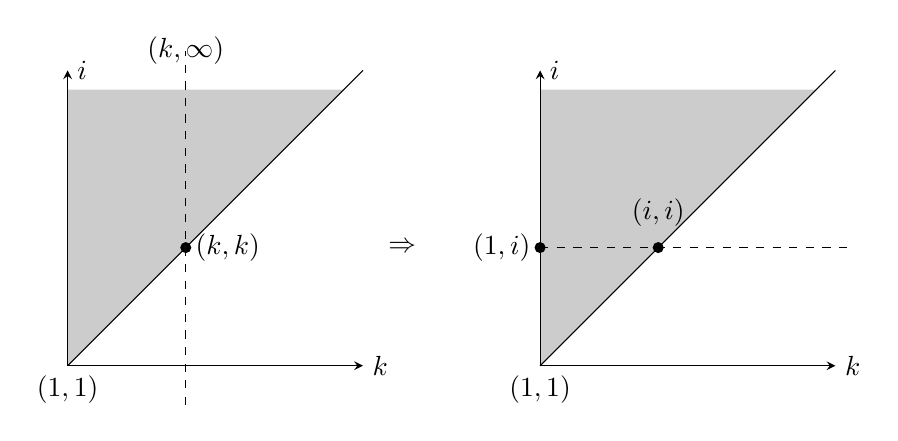
\begin{tikzpicture}[>=stealth]
    \filldraw[white!80!black] (0,0) -- (3.5,3.5) -- (0,3.5);
    \draw [->] (0,0)--(0,3.75) node [at end, right] {$i$};
    \draw  [->]  (0,0)--(3.75,0) node [at end, right] {$k$};
    \draw (0,0)--(3.75,3.75);
    \draw [dashed](1.5,-.5)--(1.5,4);
    \draw (0,0) [below] node {$(1,1)$};
    \draw (1.5,1.5) [right] node {$(k,k)$};
    \draw (1.5,4) [] node {$(k,\infty)$};
    \fill (1.5,1.5) circle (2pt);
    \draw node at (4.25,1.5) {$\Rightarrow$};
    
    \filldraw[white!80!black] (6,0) -- (9.5,3.5) -- (6,3.5);
    \draw [->] (6,0)--(6,3.75) node [at end, right] {$i$};
    \draw  [->]  (6,0)--(9.75,0) node [at end, right] {$k$};
    \draw (6,0)--(9.75,3.75);
    \draw [dashed](6,1.5)--(10,1.5);
    \draw (6,0) [below] node {$(1,1)$};
    \draw (7.5,1.65) [above] node {$(i,i)$};
    \draw (6,1.5) [left] node {$(1,i)$};
    \fill (7.5,1.5) circle (2pt);
    \fill (6,1.5) circle (2pt);
    \end{tikzpicture}
 
  
  \end{frame}



  \begin{frame}{连续型随机变量的期望}
    设$X$是有密度函数$f_X(x)$的随机变量,即密度函数满足:
    \begin{equation*}F_X(a)=\Pr(X\le a)=\int_{-\infty}^{a}f_X(x)\dif
    x \end{equation*}
    则:
    \begin{equation*}\E(X)=\int_{-\infty}^{\infty}xf_X(x)\dif x
    \end{equation*}
  
  \end{frame}


  \begin{frame}{举例:指数分布的期望}
    假设随机变量$X$服从参数为$\lambda$的指数分布,相应的概率密度函数如下:
    \begin{equation*}f_X(x)=\lambda {\rm e}^{-\lambda x}, \qquad
    \lambda>0, \;x\ge 0 \end{equation*}
      求指数分布的期望$\E(X)$。
  
  \end{frame}
  
  \begin{frame}{指数分布的期望(cont.)}
    根据期望的定义,可得:
    \begin{equation*} \E(X)=\int^{\infty}_0 x f_X(x)\dif
    x=\int^{\infty}_0 \lambda x {\rm e}^{-\lambda x}\dif
    x\end{equation*}
      记$u=-\lambda x$,则:
    \begin{equation*}\text{上式}=\frac{1}{\lambda} \int^{-\infty}_0
    u{\rm e}^{u}\dif u=\frac{1}{\lambda}\Big[{\rm
    e}^u(u-1)\Big]^{-\infty}_0=\frac{1}{\lambda}\end{equation*}
  \end{frame}



  \begin{frame}{定理}
    设$X$是非负的随机变量,则:
    \begin{equation*}
      \E(X)=\int_{0}^{\infty}\Pr(X> x)\dif
    x=\int_{0}^{\infty}\big[1-F_X(x)\big]\dif x 
  \end{equation*}

    \begin{block}{证明思路:}
      \begin{equation*}\begin{split}
        \int_{0}^{\infty}\Pr(X>x)\dif x&=\int_{0}^{\infty}\dif x
        \int_{x}^{\infty}f_X(y)\dif y=\int_{0}^{\infty}\dif
        y \underbrace{\int_{0}^{y}f_X(y)\dif x}_{\mathclap{f_X(y)\text{可从积分中提出}}}\\
        &=\int_{0}^{\infty}yf_X(y)\dif y=\E(X)\\
        \end{split}
      \end{equation*}
    \end{block}
  \end{frame}

  \subsection{方差}
  \begin{frame}{方差}
    方差(variance)是反映随机变量离散程度的指标。在概率统计的教科书中,方差计算的恒等式如下:
    \begin{equation*}{\rm Var}(X)=\E (X^2)-[\E (X)]^2 \end{equation*}
    接下来分别利用这个恒等式来计算离散型随机变量和连续型随机变量的方差。
  
  \end{frame}
  
  \begin{frame}{举例:泊松分布的方差}
    假设随机变量$X$服从参数为$\lambda$的泊松分布,相应的概率质量函数如下:
    \begin{equation*}\Pr(X=n)=\frac{\lambda^n}{n!}{\rm
    e}^{-\lambda}, \qquad \lambda>0, \;
    n=0,1,2,\ldots\end{equation*}
    求泊松分布的方差${\rm Var}(X)$。
  
    \begin{block}{思路:}
      前面已经计算出泊松分布的期望$\E(X)=\lambda$,要求出方差,还需要计算$\E( X^2)$。
    \end{block}
  \end{frame}



  \begin{frame}{泊松分布的方差(cont.)}
    \begin{equation*}\begin{split}
      \E( X^2)&= \sum_{n=0}^{\infty}n^2\Pr(X=n)= \sum_{n=0}^{\infty}
      n^2\cdot \frac{\lambda^n}{n!}{\rm e}^{-\lambda}\\
      &= \sum_{n=0}^{\infty}\frac{n\lambda^n}{(n-1)!}{\rm
      e}^{-\lambda}=\lambda {\rm e}^{-\lambda}
      \sum_{n=0}^{\infty}\frac{n\lambda^{n-1}}{(n-1)!}\\
      &=\lambda {\rm e}^{-\lambda}\cdot
      (\lambda+1){\rm e}^{\lambda} \\
      &=\lambda(\lambda+1) 
      \end{split} \end{equation*}
      因此:
      \begin{equation*}\Var(X)=\E (X^2)-[\E
      (X)]^2=\lambda(\lambda+1)-\lambda^2=\lambda \end{equation*}
  \end{frame}


  \begin{frame}{举例:指数分布的方差}
    假设随机变量$X$服从参数为$\lambda$的指数分布,相应的概率密度函数如下:
    \begin{equation*}f_X(x)=\lambda {\rm e}^{-\lambda x}, \qquad
    \lambda>0, \;x\ge 0 \end{equation*}
      求指数分布的方差$\Var(X)$。
  
      \begin{block}{思路:}
        前面已经计算出指数分布的期望$\E(X)=\dfrac{1}{\lambda}$,要求出方差,还需要计算$\E( X^2)$。
      \end{block}
  \end{frame}
  
  \begin{frame}{指数分布的方差(cont.)}
    \begin{equation*}\begin{split}
      \E( X^2)&=\int^{\infty}_0 x^2 f_X(x)\dif x=\int^{\infty}_0
      x^2\lambda {\rm e}^{-\lambda x}\dif x\\
      &=\frac{1}{\lambda}\int^{\infty}_0 (\lambda x)^2 {\rm
      e}^{-\lambda x} \dif x
        \end{split}
        \end{equation*}
      记$u=-\lambda x$,则:
      \begin{equation*}\begin{split}
      \text{上式}&= -\frac{1}{\lambda^2} \int^{-\infty}_0 u^2{\rm
      e}^u\dif u\\
      &=-\frac{1}{\lambda^2}\Big[{\rm e}^u(u^2-2u+2)
      \Big]^{-\infty}_0=\frac{2}{\lambda^2}
      \end{split} \end{equation*}
      因此:
      \begin{equation*}\Var(X)=\E (X^2)-[\E
      (X)]^2=\frac{2}{\lambda^2}-\frac{1}{\lambda^2}=\frac{1}{\lambda^2}
      \end{equation*}
  \end{frame}

  \subsection{矩母函数}

  \begin{frame}{矩母函数}
    矩母函数(moment generating function,
    mgf)是一种构造函数。对于任何满足概率密度函数为$f_X(x)$的随机变量$X$,其矩母函数的定义如下:
    \begin{equation*}
    M_X(t)=\E({\rm e}^{tX})=\int^{\infty}_{-\infty}{\rm
    e}^{tx}f_X(x)\dif x \end{equation*}
  
    根据泰勒展开式:
\begin{equation*}
{\rm
e}^x=1+x+\frac{x^2}{2!}+\frac{x^3}{3!}+\cdots=\sum^{\infty}_{k=0}\frac{x^k}{k!}
\end{equation*}
由此可得:${\rm e}^{tx}=\displaystyle\sum^{\infty}_{k=0}\frac{(tx)^k}{k!}$
  \end{frame}


  \begin{frame}{矩母函数(cont.)}
    矩母函数可以相应进行如下展开:
    \begin{equation*}\begin{split}
    M_X(t)&=\int^{\infty}_{-\infty}{\rm e}^{tx}f_X(x)\dif x
    =\int^{\infty}_{-\infty}f_X(x)\sum^{\infty}_{k=0}\frac{(tx)^k}{k!}\dif
    x \\
    &=\sum^{\infty}_{k=0}
    \frac{t^k}{k!}{\int^{\infty}_{-\infty}x^kf_X(x)\dif
    x}=\sum^{\infty}_{k=0} \frac{t^k}{k!}\cdot{\E(X^k)}\\
    &=1+t\cdot
    {\E(X)}+\frac{t^2}{2!}\cdot{\E(X^2)}+\cdots+\frac{t^n}{n!}\cdot{\E(X^n)}+\cdots
    \end{split}
    \end{equation*}
  
    由此可见,矩母函数包含了随机变量$X$的各阶矩$\E(X^n)$, $n=1,2,3,\ldots$
  \end{frame}
  
  \begin{frame}{矩母函数(cont.)}
    若对$M_X(t)$关于$t$求导,可得:
    \begin{equation*}\frac{\dif M_X(t)}{\dif
    t}=\int^{\infty}_{-\infty}{\rm e}^{tx}\cdot xf_X(x)\dif x
    \end{equation*}
    类似地:
    $$\frac{\dif^{n} M_X(t)}{\dif t^n}=\int^{\infty}_{-\infty}{\rm
    e}^{tx}\cdot x^nf_X(x)\dif x$$
    当$t=0$时:
    \begin{equation*}{\left.\frac{\dif^{n} M_X(t)}{\dif
    t^n}\right|_{t=0}}=\int^{\infty}_{-\infty} x^nf_X(x)\dif
    x=\E(X^n) \end{equation*}
    因此,可以通过对矩母函数关于$t$求$n$阶导的方式,并令$t=0$,进而求出随机变量的$n$阶矩。
  
  \end{frame}



  \begin{frame}{举例:泊松分布的各阶矩}
    假设随机变量$X$服从速率为$\lambda$的指数分布,其概率密度函数为:
    \begin{equation*}f_X(x)=\lambda {\rm e}^{-\lambda x},\qquad
    \lambda>0, \; x\ge0 \end{equation*}
      求其各阶矩。
  
      \begin{block}{思路:}
        通过矩母函数加以求解。
      \end{block}
  \end{frame}


  \begin{frame}{泊松分布的各阶矩(cont.)}
    由矩母函数的定义可得:
    \begin{equation*}\begin{split}
    M_X(t)&=\E\left({\rm e}^{tx}\right)=\int^{\infty}_0 {\rm
    e}^{tx}\lambda {\rm e}^{-\lambda x}\dif x\\
    &=\lambda \int^{\infty}_0 {\rm e}^{-(\lambda-t)x}\dif x\\
    &=\left.\frac{\lambda}{t-\lambda}{\rm
    e}^{-(\lambda-t)x}\right|^{x=\infty}_{x=0}=\frac{\lambda}{\lambda-t},\qquad
    \lambda>t
    \end{split} \end{equation*}
  \end{frame}


  \begin{frame}{泊松分布的各阶矩(cont.)}
    相应地:
    \begin{equation*}\begin{split}
    \frac{\dif M_X(t)}{\dif
    t}=\frac{\lambda}{(\lambda-t)^2}&\quad\Rightarrow\quad \E
    (X)=\left.\frac{\dif M_X(t)}{\dif
    t}\right|_{t=0}=\frac{1}{\lambda}\\
    \frac{\dif^2 M_X(t)}{\dif
    t^2}=\frac{2\lambda}{(\lambda-t)^3}&\quad\Rightarrow\quad \E
    (X^2)=\left.\frac{\dif^2 M_X(t)}{\dif
    t^2}\right|_{t=0}=\frac{2}{\lambda^2}\\
    \frac{\dif^3 M_X(t)}{\dif t^3}=\frac{2\cdot
    3\lambda}{(\lambda-t)^4}&\quad\Rightarrow\quad \E
    (X^3)=\left.\frac{\dif^3 M_X(t)}{\dif
    t^3}\right|_{t=0}=\frac{6}{\lambda^3}\\
    \end{split}\end{equation*}
    因此:$$\E (X^n)=\frac{n!}{\lambda^n}$$
  
  \end{frame}
  
  \begin{frame}{矩母函数的不足}
    通过矩母函数可以相对容易地求出服从某个概率分布的随机变量之各阶矩。但是该方法仍有不足之处,它依赖于矩母函数关于$t$进行$n$阶求导后,在$t=0$处有定义,否则会出现无法计算各阶矩的问题。

    为解决这个问题,引入特征函数(characteristic function, cf),其定义如下:
    \begin{equation*}\phi_X(t)=\E({\rm
    e}^{itx})=\int^{\infty}_{-\infty} {\rm e}^{itx}f_X(x)\dif x
    \end{equation*}
  
    特征函数的重要用途在于,若随机变量$X$的概率分布$f_X(x)$无法直接算出,可以首先计算出它的特征函数$\phi_X(t)$,再通过傅立叶变换(Fourier
transform)最终算出概率分布$f_X(x)$。
  \end{frame}

  \section{随机变量的收敛性}

  \begin{frame}{依概率收敛}
    设$\{X_n\},\;
    n\in\mathbb{N}$是一个随机变量序列。若存在一个随机变量$X$,使得$\forall\varepsilon>0$,均有:
    \[\lim_{n\to\infty}\Pr\big(|X_n-X|>\varepsilon\big)=0 \]
    则称序列$\{X_n\}$依概率收敛(convergence in probability)于$X$,记作:
    \[X_n\mathop{\longrightarrow}^P X\qquad\text{或者}\qquad
    \mathop{\rm plim}_{n\to\infty} X_n=X \]
  
    \begin{block}{}
      依概率收敛可以理解为:任意指定一个正数$\varepsilon$,无论$n$取多大,$X_n$与$X$差距的绝对值大于$\varepsilon$的可能次数仍然是存在的,但只要$n$足够大,这种例外情形的次数占比将逐渐趋于0。
    \end{block}
  \end{frame}

  \begin{frame}{弱大数定律}
    设$\{X_n\}$是一个随机变量序列,$\E(X_n)$存在。令$\bar
    X_n=\displaystyle\frac{1}{n}\sum^n_{i=1}X_i$,若
    \[\bar X_n-\E(\bar X_n)\mathop{\longrightarrow}^P 0 \]
    则称随机变量序列$\{X_n\}$服从弱大数定律(weak law of large numbers)。
  \end{frame}




  \begin{frame}{以概率1收敛}
    设$\{X_n\},\; n\in\mathbb{N}$是一个随机变量序列,若存在一个随机变量$X$,使得
    \[\lim_{n\to\infty}\Pr\left(\bigcup^{\infty}_{i=n}|X_i-X|>\varepsilon\right)=0
    \]
    则称序列$\{X_n\}$以概率1收敛(convergence with probability 1)于$X$,
    也称作“几乎处处收敛”(almost surely convergence),
    记作:$$X_n\displaystyle\mathop{\longrightarrow}^{\rm a.s.}
    X,\qquad \text{或}\qquad X_n\to X, \quad \text{a.s.}$$
    
    该定义的等价形式是:
    \[\Pr\left(\lim_{n\to\infty}X_n=X\right)=1 \]
  \end{frame}


  \begin{frame}{以概率1收敛(cont.)}
    \begin{block}{}
      以概率1收敛可以理解为:只要$n$足够大,任意指定一个正数$\varepsilon$,总能找到一个$N$,使得$n>N$时,$X_n$与$X$差距的绝对值不再
大于$\varepsilon$。正因如此,以概率1收敛比依概率收敛的条件强,也就是说以概率1收敛意味着一定依概率收敛,反之则不然。
    \end{block}
  \end{frame}
  
  \begin{frame}{强大数定律}
    设$\{X_n\}$是一个随机变量序列,$\E(X_n)$存在。令$\bar
    X_n=\displaystyle\frac{1}{n}\sum^n_{i=1}X_i$,若
    \[\bar X_n-\E(X_n)\mathop{\longrightarrow}^{a.s.} 0\qquad
    \text{或}\qquad \Pr\left[\lim_{n\to\infty}\bar
    X_n=\E(X_n)\right]=1 \]
    则称随机变量序列$\{X_n\}$服从强大数定律(strong law of large numbers)。
  
\begin{block}{}
  所谓大数定律,实际上是想要说明当对一个随机变量进行无限次采样时,得到的平均值会无限接近真实的
期望值。只不过强大数定律是想说明,采样的次数越多,平均值几乎一定越接近真实期望值(这意味着不可能出现反方向的偏离);
而弱大数定律则是想说明,采样的次数越多,平均值接近真实期望值的可能性越大(这意味着也有极小的可能出现反方向的偏离)。
\end{block}

  \end{frame}



 


  \begin{frame}{柯尔莫哥洛夫(Kolmogorov)大数定律}
    设$\{X_n\}$是相互独立的随机变量序列,并且$\displaystyle\sum^{\infty}_{k=1}\frac{\Var(X_k)}{k^2}<\infty$,则$\{X_n\}$服从强大数定律,即:
    \[\Pr\left\{\lim_{n\to\infty}\frac{1}{n}\sum^{\infty}_{k=1}[X_k-\E(X_k)]=0
    \right\}=1 \]
  \end{frame}



 


  \begin{frame}{柯尔莫哥洛夫大数定律(cont.)}
    更进一步,在柯尔莫哥洛夫大数定律的基础上,假设$\{X_n\}$同分布,并且$\E(X_n)=\mu$,令$\bar
X_n=\displaystyle\frac{1}{n}\sum^n_{i=1}X_i$,则:
\[\Pr\left(\lim_{n\to\infty} \bar X_n=\mu  \right)=1 \]
换句话说,如果随机变量序列$\{X_n\}$独立同分布(independent and identically
distributed, iid),则随着样本的增大,样本的均值将以概率1收敛于总体的均值。
这是后面研究随机过程性质的重要基础。
  \end{frame}
  
  \begin{frame}{均方收敛}
    设$\{X_n\},\; n\in\mathbb{N}$是一个随机变量序列,$X$是一个随机变量。若
    \[\lim_{n\to\infty}\E\big[(X_n-X)^2\big]=0 \]
    则称序列$\{X_n\}$均方收敛(convergence in mean square)于$X$,
    记作:
    \[X_n\mathop{\longrightarrow}^{\rm m.s.} X\]
  
    \begin{block}{注意:}     
均方收敛是从随机变量的二阶矩的角度考虑收敛问题,其约束很严格,且不能与以概率1收敛互相推导。
    \end{block}
  \end{frame}



  \begin{frame}{依分布收敛}
    设$\{F_n(x)\}$是随机变量序列$\{X_n\},\;
    n\in\mathbb{N}$的分布函数列,如果存在一个单调不减函数$F(x)$,使得在$F(x)$所有的连续点$x$上,有:
    \[\lim_{n\to\infty}F_n(x)=F(x) \]
    则称随机变量序列$X_n$依分布收敛(convergence with distribution)于$X$,记作:
    \[X_n\mathop{\longrightarrow}^L X \]
    称函数列$\{F_n(x)\}$弱收敛于$F(x)$。
  
    \begin{block}{}
      依分布收敛的约束非常小,此种形式的收敛并未考虑随机变量的值,只考察两者的分布函数是否相近。
    \end{block}
  \end{frame}


  \begin{frame}{几种收敛的关系}
    \centering
    \begin{tikzpicture}[>=stealth]
      \node (s1) at (0,0)[rectangle,draw=blue!50,fill=blue!20] {均方收敛};\node (s2) at (4,0)[rectangle,draw=blue!50,fill=blue!20]
      {以概率1收敛};
      \node (s3) at (2,-2)[rectangle,draw=blue!50,fill=blue!20]
      {依概率收敛};
      \node (s4) at (2,-4)[rectangle,draw=blue!50,fill=blue!20]
      {依分布收敛};
        \draw [->] (s1.south) -- (s3);
        \draw [->] (s2.south) -- (s3);
        \draw [->] (s3.south) -- (s4.north);
        
        \end{tikzpicture}
  
  \end{frame}
  

  \section{随机过程的概念}
  \begin{frame}{随机过程的概念}
    设$(\Omega,\mathcal{F},\Pr)$是一个概率空间,$T$为一个参数集。若对每一个$t\in
    T$,均有定义在概率空间上的一个随机变量$X_t(\omega),\;
    \omega\in\Omega$与之对应,则称$\{X_t:t\in
    T\}$为$(\Omega,\mathcal{F},\Pr)$上的一个随机过程(stochastic process)。
    这里的$t$通常理解成时间,相应的参数集$T$就是时间参数;$X_t$可看作过程在时刻$t$的状态。$X_t$的取值范围称作状态空间$\Omega$。
    
  
  \end{frame}



  \begin{frame}{随机过程的概念(cont.)}
    对于$X_t(\omega)$,
  \begin{itemize}
    \item 若固定$\omega$,则$X_t$称为样本函数或轨道,是随机过程的一次实现(realization);
    \item 若固定$t$,则$X(\omega)$称为一个随机变量;
    \item 所有可能出现的结果的总体$\{X_1(\omega),X_2(\omega),\ldots,X_n(\omega),\ldots\}$,
    $\omega\in\Omega$构成一个随机过程。
  \end{itemize}

  随机过程这个词包含了两重含义:“随机”意味着某时刻出现结果的不确定性,但是可能的结果一定在状态空间内;“过程”意味着还要考虑
随机现象随时间的演化规律。正因如此,随机过程可看作所有样本函数的集合(assemble)。
  \end{frame}


  \begin{frame}{以股价为例说明随机过程的含义}
  \centering  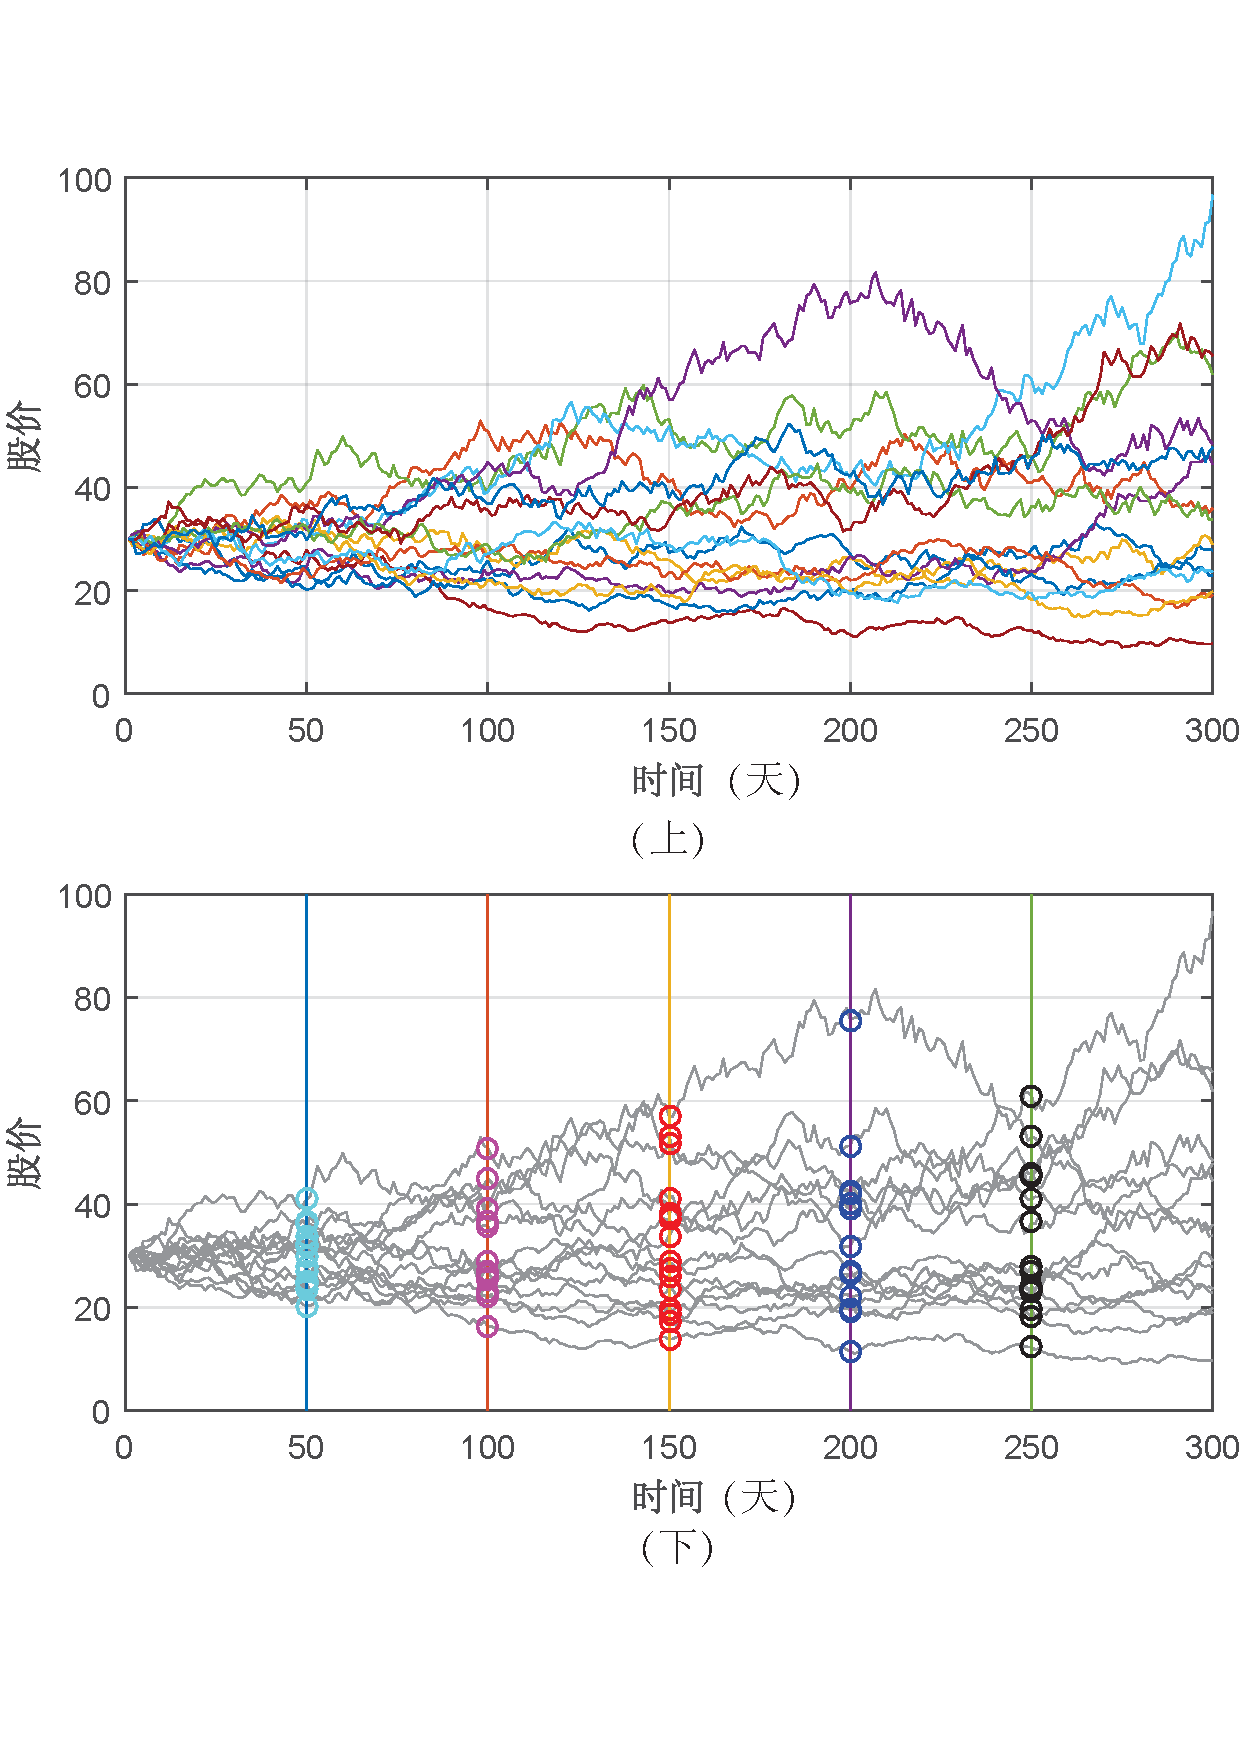
\includegraphics[scale=.3]{fig/stk.pdf}
  
  \end{frame}
  
















\end{document}